\documentclass[12pt]{article}
\usepackage{listings}
\usepackage[pdftex]{graphicx}
\usepackage[colorlinks=true,pagebackref,linkcolor=blue]{hyperref}
\textwidth=7in
\textheight=9.5in
\topmargin=-1in
\headheight=0in
\headsep=.5in
\hoffset  -.85in

\lstset{
basicstyle=\footnotesize\ttfamily,
language=bash,
upquote=true,
breakatwhitespace=true,
columns=fullflexible,
keepspaces,
%numbers=none,
tabsize=3,
frame=blrt,
framextopmargin=5pt,
showstringspaces=false,
extendedchars=true
}

\pagestyle{empty}

\renewcommand{\thefootnote}{\fnsymbol{footnote}}

\begin{document}



\begin{center}
{\bf AMS 550.400 \quad HW SET 1\quad  Name: Joyce Tan}\\
\vskip.2in

\end{center}

\setlength{\unitlength}{1in}

\begin{picture}(6,.1) 
\put(0,0) {\line(1,0){6.25}}         
\end{picture}

 

\renewcommand{\arraystretch}{2}


\vskip.25in
\noindent\textbf{Problem 1 (10 pts):}  

\noindent\verb+mkdir abc.git+
\\*\verb+cd abc.git+
\\*\verb+git init .+
\\*\verb+vi main.txt+
\\*\verb+git add .+
\\*\verb+git commit -m "A done"+
\\*\verb+vi main.txt+
\\*\verb+git add .+
\\*\verb+git commit -m "B done"+
\\*\verb+git branch alt+
\\*\verb+vi main.txt+
\\*\verb+git add .+
\\*\verb+git commit -m "C done"+
\\*\verb+git checkout alt+
\\*\verb+vi main.txt+
\\*\verb+git add .+
\\*\verb+git commit -m "X done"+
\\*\verb+git checkout master+
\\*\verb+git merge alt+
\\\*\verb+vi main.txt+
\\*\verb+git add .+
\\*\verb+git commit -m "merge"+
\\\*\verb+vi main.txt+
\\*\verb+git add .+
\\*\verb+git commit -m "done"+
\\*\verb+git log --graph --oneline+
\\*\verb+git checkout alt+
\\*\verb+git log --graph --onelinee+


\vskip0.25in Fig 1. Master Graph
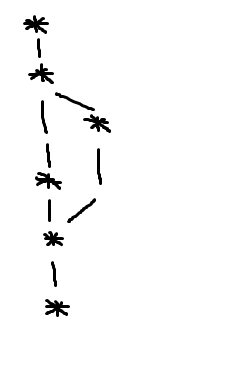
\includegraphics{fig1.png}

\vskip.25in Fig 2. Branch graph
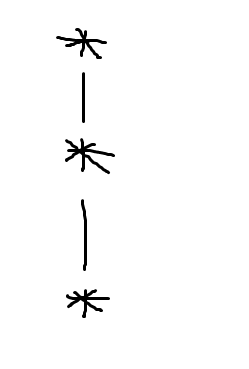
\includegraphics{fig2.png}

\vskip.25in
\noindent\textbf{Problem 2 (10 pts):}
\noindent
\\*\verb+git config --global user.name "Joyce Tan"+
\\*\verb+git confit --global user.email jtan21@jhu.edu+
\\*\verb+git add remote x1 git://github.com/nhlee/550400.stanza1.git+
\\*\verb+git add remote x2 git://github.com/nhlee/550400.stanza2.git+
\\*\verb+git add remote x3 git://github.com/nhlee/550400.stanza3.git+
\\*\verb+mkdir poem.git+
\\*\verb+cd poem.git+
\\*\verb+git init .+
\\*\verb+git pull x1 master+
\\*\verb+vi main.txt+
\\*\verb+git pull x2 master+
\\*\verb+git pull x3 master+
\\*\verb+vi main.txt+
\\*\verb+git add .+
\\*\verb+git commit -m "done"+
\\*\verb+git add remote origin https://github.com/jtan21/poemmerge.git+
\\*\verb+git push origin master+


\newpage
\noindent\textbf{Problem 3 (40 pts):}
\vskip0.25in Team projects are always a difficult issue since it is almost impossible to find a way to coordinate meeting and discussion times. This process can potentially be time-consuming, and an negative impact on the working relationship between the team members. If handled in an inefficient way, the project is unlikely to fulfill its full potential. In this case, we are considering a team of 4 students (“A”, “B”, “C”, and “D”) who are working on writing a latex/beamer file (“main.tex”) for a class presentation of their work statement. Specifically, A is in charge of the Introduction/Preamble, B is in charge of the Problem Statement, C is in charge of the Timeline, and D is in charge of the Deliverables. They do not wish to coordinate their schedules for a concurrent group meeting, either virtually or in person. In terms of their work allocations, their contributions to main.tex do not overlap. We want to devise two work flow strategies for the team so that they can collaborate asynchronously using git. We will then compare the two strategies and make a final recommendation. 
\vskip0.25in The exogenous variables are the four contributions from the four  members of the team, since they are the inputs for the strategy. These exogenous variables combine to form the final product, which is the merged main.tex. The endogenous variable is the work flow strategy we are suggesting. Unimportant variables include the length of each contribution and the sequence in which the contributions are compiled. The preamble part of main.tex is also exogenous since it only needs to be entered once to produce main.tex.
\vskip0.25in The first strategy is to create a central repository, and have all four members create their own respective repositories. The 4 people should work on their individual portions separately and then push it to their own repositories. When they have finalized their individual parts and pushed it, the leader can pull the separate portions and merge it to a main main.tex. The merging should be pretty straightforward since none of 4 parts overlap as they are all working on separate sections. Also, before they finalize their individual parts they can get comments by providing the repositories'' address to their other members. The only concern would be to ensure that the main.tex of the main repository is correctly merged. 
\vskip0.25in The second strategy is to create a single central repository, and create four branches, one for each member. Each individual would be working from their individual branches, they can copy the format from the master branch. Once they have finalized their individual parts, the leader can go to the master branch, and merge the other 4 branches one at a time. The project can be assembled by removing any conflicts. 
\vskip0.25in Both models are useful, since it manages to allow the individual students work on their part without any interference from other team members. It will also allow the leader to merge all the different sections to form one collated version of main.tex. Thus this model is useful.
\vskip0.25in These models can be tested out, by asking each student to write 2 lines of a poem. The goal would be then to assemble the entire poem. The students can test out the 2 strategies, to see if the process is simple enough and if it obtains the desired result easily.
\vskip0.25in Now that we have 2 working strategies, we need to evaluate which would be a better choice. Regarding merge conflicts, both strategies would have the same issues, since merging from a branch and pulling from a repository does not make a difference. The first strategy which utilizes different repositories is a little more tedious in the sense the each member has to constantly push their document to the repository if they want to allow the other members to view their work so far. This would not be a problem for the second strategy since all changes can be viewed once the document is saved.  Thus I recommend the second strategy, since it is important to keep track of what other members are working on, such that the entire project can be as cohesive as possible.


d 

\vskip0.25in
\noindent\textbf{Problem 4 (aka.\ Fair Play, 40 pts):}
\vskip0.25in Is the tennis game fair? To answer this question, we have to define what fair means. This is the problem statement: No matter if a player serves first or second, his probability of winning the entire match is 0.5. We have to make many assumptions to build this model. We assume that both players are equally skilled, have the same skill set (offensive and defensive), and that serving first gives an advantage in winning that point. 
\vskip0.25in In order to proved, we have to clarify the point system of a tennis match. A tennis match is composed of points, games and sets. Assuming a best of 5 format, a player has to win 3 sets to win the match. To win a set, a player has to be the first to win at least 6 games and by at least 2 games. If both players have won 6 games each in a single set, they head for a tiebreak where the player wins the set by scoring at least 7 points and winning by at least 2 points in this tiebreak game. The player who is supposed to serve in the next game serves in this tiebreak game. In a normal non-tiebreak game, players win the game by scoring at least 4 points and by at least 2 points. 
\vskip0.25inGiven this information, the exogenous variables are the points, games, sets and to whom the service is awarded to in each of these, whether it is player A or player B.  The endogenous variable will be the winner of the match, given whether player A or player B serves. 
\vskip0.25inTo make it easier to visualize, we assume that serving a game is advantageous, and a player is sure to win the game if he starts serving first. If player 1 serves first, he will win the first set (1-0), However, player 2 will serve the second set and equalize the score (1-1). This will go on until both players are tied 6-6, since player 2 will keep equalizing any point that player 1 wins. In a tiebreak game, player 1 serves first and will win the first point. Player 2 will then serve the next 2 points and it will be 3-2. Player 1 has 2 turns next to serve and it will be 3-4. It will keep equalizing by twos in this manner and there is no way for either player to win by 2 points to break this tie.  Considering that there is no causal relationship between a player's performance and the previous point (no psychological/tiredness effect), the tiebreak structure (need to win by at least 2 points) prevents any unfair advantage from serving first, if both players are equally matched in skill.
\vskip0.25in However, it is likely that there does exist a correlation between a player's performance and the result of the previous point played. One might be highly motivated to perform even better if he performs well in the previous set. He might also be spurred to perform better if he lost the previous set. This correlation is highly qualitative and depends on the players' psychological mentality.There are also many other factors that come into effect regarding the advantage of serving first. If one is a defensive player, it might be more advantageous to serve second, or if one has a weak serve, it is impossible to determine if one will surely win the game if one serves it. Thus, modeling this problem is not very useful as it does not provide much information. Also, since there are so many assumptions, it is difficult to have any concrete conclusions from this. 
\vskip0.25in We can also attempt to test this model out, to see if there is a differet whether a player serves first. According to our theory, it should not make a differentiate whether or not a player serves first. We could try to pitch 2 players of the same level against each other and make them play many matches. However this is not practical. Alternatively, we can look at results of past tennis matches against the top players in the world, since they should be pretty much equally matched. However this might also not be very accurate, as it would be difficult to determine if they have similar styles of playing (offensive/defensive etc).
\vskip0.25in This model would be more conclusive if we can somehow quantify the behavior of all players depending on the performance of the previous set. Then again, it is difficult to lump all players into one category and at the end of the day, the game favors the player who can perform well despite the circumstanfes, no matter the result of the previous point. Thus, in this sense, tennis is fair, since serving first does not offer any significant advantage. 


\end{document}
